\حصہء{سوالات}
\موٹا{محددی لکیر پر حرکت}\\
سوال \حوالہ{سوال_تفرق_محددی_لکیر_الف} تا سوال \حوالہ{سوال_تفرق_محددی_لکیر_ب} میں \عددی{a\le t\le b} کے لئے \عددی{s=f(t)} محددی لکیر پر ایک جسم کا مقام دیتی ہے جہاں \عددی{t} کی اکائی سیکنڈ اور \عددی{s} کی اکائی میٹر ہے۔
\begin{enumerate}[a.]
\item
دیے گئے وقفے پر جسم کا ہٹاو اور سمتی رفتار حاصل کریں۔
\item
اس وقفے کے  آخری سروں پر جسم کی رفتار اور اسراع تلاش کریں۔
\item
جسم کب حرکت کی سمت تبدیل کرتا ہے (اگر ایسا کرتا ہو)؟   
\end{enumerate}

\ابتدا{سوال}\شناخت{سوال_تفرق_محددی_لکیر_الف}
$s=0.8t^2,\quad 0\le t\le 10 \quad \text{\RL{چاند پر آزادانہ گرنا}}$
\انتہا{سوال}
%======================
\ابتدا{سوال}
$s=1.86t^2,\quad 0\le t\le 0.5\quad \text{\RL{مریخ پر آزادانہ گرنا}}$
\انتہا{سوال}
%========================
\ابتدا{سوال}
$s=-t^3+3t^2-3t,\quad 0\le t\le 3$
\انتہا{سوال}
%=========================
\ابتدا{سوال}
$s=\tfrac{t^4}{4}-t^3+t^2,\quad 0\le t\le 2$
\انتہا{سوال}
%=========================
\ابتدا{سوال}
$s=\tfrac{25}{t^2}-\tfrac{5}{t},\quad 1\le t\le 5$
\انتہا{سوال}
%========================
\ابتدا{سوال}\شناخت{سوال_تفرق_محددی_لکیر_ب}
$s=\tfrac{25}{t+5},\quad -4\le t\le 0$
\انتہا{سوال}
%========================
\ابتدا{سوال}
\عددی{s} محور پر لمحہ \عددی{t} پر  ایک جسم کا مقام \عددی{s=t^3-6t^2+9t} ہے۔ (ا) ان نقطوں پر اس جسم کی اسراع تلاش کریں جن پر جسم کی سمتی رفتار صفر ہو گی۔ (ب) جب جسم کی اسراع صفر ہو اس لمحے پر اس جسم کی رفتار کیا ہو گی؟ (ج) لمحہ \عددی{t=0} تا \عددی{t=2} کے دوران یہ جسم کل کتنا فاصلہ طے کرتی ہے۔
\انتہا{سوال}
%==========================
\ابتدا{سوال}
وقت \عددی{t\ge 0} پر \عددی{s} محور پر حرکت کرتے ہوئے جسم کی سمتی رفتار \عددی{v=t^2-4t+3} ہے۔ (ا) جسم کی اسراع وہاں تلاش کریں جہاں جسم کی سمتی رفتار صفر ہے۔ (ب)  جسم کب آگے رخ اور کب پیچھے رخ حرکت کرتی ہے؟ (ج) جسم کی سمتی رفتار کب بڑھتی اور کب گھٹتی ہے؟
\انتہا{سوال}
%============================
\موٹا{آزادانہ گرنا}

\ابتدا{سوال}
مریخ اور مشتری کی سطح کے قریب آزادانہ گرنے کے مساوات بالترتیب \عددی{s=1.86t^2} اور \عددی{s=11.44t^2} ہیں جہاں \عددی{t} کی اکائی سیکنڈ اور \عددی{s} کی اکائی میٹر ہے۔ ساکن حال سے گرتے ہوئے کتنے وقت میں (مریخ اور مشتری میں) ایک جسم کی رفتار \عددی{\SI{27.8}{\meter\per\second}} یعنی تقریباً \عددی{\SI{100}{\kilo\meter\per\hour}} ہو گی؟
\انتہا{سوال}
%========================
\ابتدا{سوال}\شناخت{سوال_تفرق_پتھر_مریخ}
سطح چاند سے  انتصابی رخ \عددی{\SI{25}{\meter\per\second}} کی رفتار سے  پھینکا گیا پتھر \عددی{t} سیکنڈوں میں \عددی{s=24t-0.8t^2} میٹر بلندی پر پہنچے گا۔
\begin{enumerate}[a.]
\item
لمحہ \عددی{t} پر پتھر کی اسراع کیا ہو گی؟ (یہ اسراع چاند پر کشش ثقل کی اسراع ہو گی۔)
\item
پتھر بلند ترین مقام تک کتنے دورانیے میں پہنچے گا؟
\item
پتھر کتنی بلندی تک پہنچ پائے گا؟
\item
بلند ترین مقام کی نصف تک پتھر کتنی دیر میں پہنچے گا؟
\item
پتھر  کتنے وقت میں سطح چاند پر گرے گا؟ 
\end{enumerate}   
\انتہا{سوال}
%=========================
\ابتدا{سوال}
سطح زمین پر ہوا کی  غیر موجودگی میں سوال \حوالہ{سوال_تفرق_پتھر_مریخ} کا پتھر \عددی{t} سیکنڈوں میں \عددی{s=24t-4.9t^2} بلندی پر ہو گا۔
\begin{enumerate}[a.]
\item
لمحہ \عددی{t} پر پتھر کی اسراع کیا ہو گی؟ (یہ اسراع چاند پر کشش ثقل کی اسراع ہو گی۔)
\item
پتھر بلند ترین مقام تک کتنے دورانیے میں پہنچے گا؟
\item
پتھر کتنی بلندی تک پہنچ پائے گا؟
\item
بلند ترین مقام کی نصف تک پتھر کتنی دیر میں پہنچے گا؟
\item
پتھر  کتنے وقت میں سطح چاند پر گرے گا؟ 
\end{enumerate}   
\انتہا{سوال}
%========================
\ابتدا{سوال}
ہوا سے خالی ایک دنیا پر ایک ٹھوس جسم کو انتصابی رخ \عددی{\SI{15}{\meter\per\second}} کی ابتدائی رفتار سے پھینکا گیا۔ اس دنیا کے سطح پر ثقلی اسراع  \عددی{g_s \,\si{\meter\per\second\squared}} ہونے کی بنا \عددی{t} سیکنڈوں میں جسم \عددی{s=15t-\tfrac{1}{2}g_st^2}  میٹر بلندی تک پہنچے گا۔یہ جسم بلند ترین مقام تک \عددی{20} سیکنڈوں میں پہنچتا ہے۔ اس دنیا میں ثقلی اسراع کتنی ہے؟
\انتہا{سوال}
%==========================
\ابتدا{سوال}
چاند پر ایک بندوق کو انتصابی رخ چلایا گیا۔بندوق کی گولی \عددی{t} سیکنڈوں میں \عددی{s=300t-4.9t^2} میٹر بلندی پر ہو گی۔چاند پر یہی گولی \عددی{t} سیکنڈ بعد \عددی{s=300t-0.8t^2} میٹر بلندی پر ہو گی۔دونوں صورتوں میں گولی کتنی دیر بعد سطح پر گرے گی؟
\انتہا{سوال}
%=============================
\ابتدا{سوال}
مشتری پر ہوا کی غیر موجودگی میں یہی گولی \عددی{t} سیکنڈ بعد \عددی{s=300t-11.44t^2} میٹر بلندی پر ہو گی جبکہ مریخ پر یہ \عددی{s=300t-1.86t^2} میٹر کی بلندی پر ہو گی۔دونوں صورتوں میں گولی کتنے بلندی تک پہنچے گی؟
\انتہا{سوال}
%=================
\ابتدا{سوال}\شناخت{سوال_تفرق_تجربہ_گلیلو}\ترچھا{گلیلو کا کلیہ برائے آزادانہ گرنا}
ایک پٹی کو مختلف زاویوں پر رکھتے ہوئے گلیلو نے اس پر گیند کی سمتی رفتار کو ناپتے ہوئے کلیہ اخذ کیا جس کی تحدیدی صورت سے آزادانہ گرتے ہوئے جسم کی سمتی رفتار کا کلیہ حاصل کرنا مقصد تھا (شکل \حوالہ{شکل_سوال_تفرق_تجربہ_گلیلو})۔گلیلو نے دیکھا کہ حرکت کے شروع سے \عددی{t} سیکنڈ بعد سمتی رفتار کی قیمت \عددی{t} کے راست متناسب ہے یعنی  \عددی{v=kt} لکھا جا سکتا ہے۔ مستقل \عددی{k} کی قیمت کا دارومدار پٹی کی ڈھلوان پر ہے۔
\begin{figure}
\centering
\begin{subfigure}[b]{0.45\textwidth}
\centering
\begin{tikzpicture}
\draw(-2,0)--(4,0);
\draw[thick](0,0)--++(160:2)coordinate[pos=0.8](kA);
\draw(kA)++(160-90:0.25)circle(0.25);
\draw[thick](1,0)--++(140:2)coordinate[pos=0.8](kA);
\draw(kA)++(140-90:0.25)circle(0.25);
\draw[thick](2,0)--++(120:2)coordinate[pos=0.8](kA);
\draw(kA)++(120-90:0.25)circle(0.25);
\draw[thick,dashed](3,0)--++(90:2)coordinate[pos=0.8](kA)node[above,solid,align=right]{\RL{آزادانہ گرنے}\\ \RL{کا مقام}};
\draw[dashed](kA)++(90-90:0.25)circle(0.25);
\end{tikzpicture}
\caption{}
\end{subfigure}%
\begin{subfigure}[b]{0.45\textwidth}
\centering
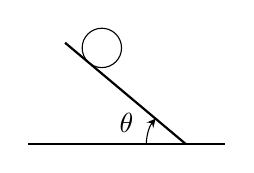
\begin{tikzpicture}
\draw(-0.5,0)--(2,0);
\draw[thick](1.5,0)--++(140:2)coordinate[pos=0.8](kA);
\draw(kA)++(140-90:0.25)circle(0.25);
\draw[stealth-]([shift={(140:0.5)}]1.5,0) arc (140:180:0.5);
\draw(1.5,0)++(160:0.8)node[]{$\theta$};
\end{tikzpicture}
\caption{}
\end{subfigure}%
\caption{گلیلو کا تجربہ برائے آزادانہ گرنا (سوال \حوالہ{سوال_تفرق_تجربہ_گلیلو})}
\label{شکل_سوال_تفرق_تجربہ_گلیلو}
\end{figure}  

موجودہ علامتیت استعمال کرتے ہوئے (شکل \حوالہ{شکل_سوال_تفرق_تجربہ_گلیلو}-ب)  درحقیقت گلیلو نے درج ذیل کلیہ حاصل کیا تھا جہاں فاصلے کی اکائی میٹر اور وقت کی اکائی سیکنڈ ہے۔
\begin{align*}
v=(9.8\sin \theta)t
\end{align*} 
(ا) آزادانہ گرتے ہوئے گیند کی رفتار کیا ہو گی؟ (ب) سطح زمین کے قریب جسم کی اسراع کیا ہو گی؟
\انتہا{سوال}
%=======================
\ابتدا{سوال}\ترچھا{پی سا}
اگر گلیلو پی سا سے توپ کی گولی \عددی{\SI{55}{\meter}} بلندی سے گرنے دیتا تب \عددی{t} سیکنڈ بعد سطح زمین سے اس کی بلندی \عددی{s=55-4.9t^2} ہوتی۔ (ا) لمحہ \عددی{t} پر توپ کی گولی کی سمتی رفتار، رفتار اور اسراع کیا ہوتے؟ (ب) یہ زمین تک کتنی دیر میں پہنچتا؟ (ج) زمین پر پہنچنے کے لمحہ پر اس کی سمتی رفتار کیا ہوتی؟ 
\انتہا{سوال}
%=============================
\موٹا{ترسیم سے حرکت کے بارے میں معلومات اخذ کرنا}

\ابتدا{سوال}
ایک محوری لکیر پر ایک جسم کی سمتی رفتار \عددی{v=\tfrac{\dif s}{\dif t}=f(t)} کو درج ذیل شکل میں ترسیم کیا گیا ہے۔
\begin{centering}
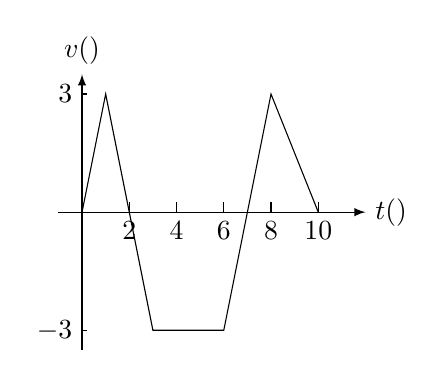
\begin{tikzpicture}[x={0.3cm},y={0.5cm}]
\draw[-latex](-1,0)--(12,0)node[right]{$t(\si{\second})$};
\draw[-latex](0,-3.5)--(0,3.5)node[above]{$v(\si{\meter\per\second})$};
\draw(0,0)--(1,3)--(3,-3)--(6,-3)--(8,3)--(10,0);
\foreach \x in {2,4,6,8,10}{\draw(\x,0)node[below]{$\x$}--++(0,0.25);}
\foreach \y in {-3,3}{\draw(0,\y)node[left]{$\y$}--++(0.2,0);}
\end{tikzpicture}
\end{centering}
(ا) جسم کب سمت حرکت تبدیل کرتی ہے؟ (ب) کب جسم تقریباً مستقل رفتار سے حرکت کرتی ہے؟ (ج) دورانیہ \عددی{0\le t\le 10} کے لئے جسم کی رفتار ترسیم کریں۔ (د) جسم کی اسراع (جہاں معین ہو) ترسیم کریں۔
\انتہا{سوال}
%============================
\ابتدا{سوال}\شناخت{سوال_تفرق_محوری_لکیر_پر_حرکت}
ایک محوری لکیر پر  نقطہ \عددی{N} حرکت کرتا ہے۔اس نقطے  کا مقام بالمقابل وقت بھی ترسیم کیا گیا ہے (شکل \حوالہ{شکل_سوال_تفرق_محوری_لکیر_پر_حرکت})۔ (ا) \عددی{N} کب بائیں رخ حرکت کرتا ہے؟ کب دائیں رخ حرکت کرتا ہے؟ کب ساکن ہے؟ (ب) اس کی سمتی رفتار اور رفتار (جہاں معین ہوں) ترسیم کریں۔ 
\begin{figure}
\centering
\begin{subfigure}{0.45\textwidth}
\centering
\begin{tikzpicture}
\draw[-latex](-0.5,0)--(3,0)node[right]{$s(\si{\centi\meter})$};
\draw(0,0)node[below]{$0$}--++(0,0.1) (1.5,0)node[circ]{}node[above]{$N$};
\end{tikzpicture}
\caption{}
\end{subfigure}\hfill
\begin{subfigure}{0.45\textwidth}
\centering
\begin{tikzpicture}
\begin{axis}[small,axis lines=middle,xlabel={$t(\si{\second})$},ylabel={$s(\si{\centi\meter})$},xtick={1,2,3,4,5,6},ytick={-4,-2,2},ymin=-5,ymax=4,xmax=9]
\addplot[] plot coordinates {(0,0) (1,2) (2,2) (3,-2) (5,-2) (6,-4)};
\draw(axis cs:6,-4)node[circ]{}node[right]{$(6,-4)$};
\draw(axis cs:4,2)node[]{$s=f(t)$};
\end{axis}
\end{tikzpicture}
\caption{}
\end{subfigure}
\caption{محوری لکیر پر حرکت (سوال \حوالہ{سوال_تفرق_محوری_لکیر_پر_حرکت})}
\label{شکل_سوال_تفرق_محوری_لکیر_پر_حرکت}
\end{figure}
\انتہا{سوال}
%============================
\ابتدا{سوال}\شناخت{سوال_تفرق_راکٹ}
راکٹ میں چند سیکنڈوں کے لئے ایندھن ہوتا ہے جو اس کو کسی خاص بلندی تک پہنچاتا ہے جس کے بعد راکٹ کچھ دیر تک مزید بلند ہو کر واپس زمین کی جانب گرتا ہے۔گرنے کے چند لمحات بعد خود کار پیراشوٹ کھلتا ہے جو راکٹ کو حفاظت کے ساتھ نہایت آہستہ زمین تک پہنچاتا ہے۔ ایک راکٹ کی حرکت کو شکل \حوالہ{شکل_سوال_تفرق_راکٹ} میں ترسیم کیا گیا ہے۔ (ا) ایندھن ختم ہونے کے لمحہ راکت کی رفتار کتنی تھی؟ (ب) ایندھن کتنے سیکنڈوں تک کے لئے تھا؟ (ج)  راکٹ کب بلند ترین مقام تک پہنچا اور بلند ترین مقام پر اس کی رفتار کتنی تھی؟ (د) پیراشوٹ کب کھلا اور اس لمحہ پر راکٹ کی رفتار کتنی تھی؟ (ہ) پیرا شوٹ کھلنے سے پہلے راکٹ کتنی دیر تک گرتا رہا؟ (و) راکٹ کی اسراع کب زیادہ سے زیادہ تھی؟ (ز) اسراع کب مستقل تھی اور اس کی قیمت کیا تھی؟\\
جواب:\quad
(ا) \عددی{\SI{60}{\meter\per\second}} (ب) \عددی{\SI{2}{\second}} (ج) \عددی{t=\SI{8.12}{\second}}، \عددی{v=\SI{0}{\meter\per\second}} (د) \عددی{\SI{12}{\second}}، \عددی{v=\SI{-38}{\meter\per\second}} (ہ) \عددی{\SI{10}{\second}} (و) لمحہ \عددی{t=\SI{2}{\second}} پر (ز) \عددی{\SI{2}{\second}} تا \عددی{\SI{12}{\second}}
\begin{figure}
\centering
\begin{minipage}{0.45\textwidth}
\centering
\begin{tikzpicture}
\begin{axis}[clip=false,small,axis lines=middle,xmax=17,ymin=-40,ymax=70,xmax=20,ytick={-38,-5,60},xtick={2,8.12,12,17},xlabel={$t(\si{\second})$},ylabel={$v(\si{\meter\per\second})$},ylabel style={at={(current axis.above origin)},anchor=south},xlabel style={at={(current axis.right of origin)},anchor=west}]
\pgfmathsetmacro{\k}{0.15}
\addplot[domain=0:2]{12*x/(1-0.3*x)};
\addplot[domain=0:10]({x+2},{60-9.8*x});
\draw(axis cs:12,-38) to [out=70,in=-180](axis cs:17,-5);
\end{axis}
\end{tikzpicture}
\caption{راکٹ کی حرکت (سوال \حوالہ{سوال_تفرق_راکٹ})}
\label{شکل_سوال_تفرق_راکٹ}
\end{minipage}\hfill
\begin{minipage}{0.45\textwidth}
\centering
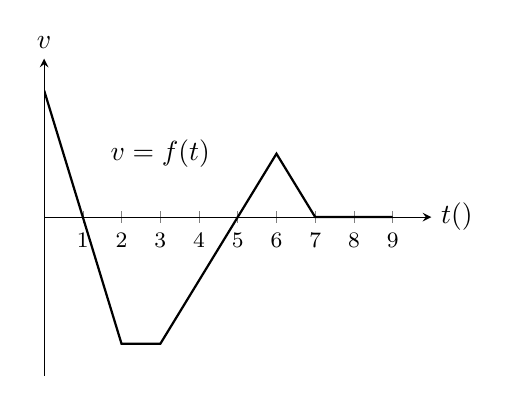
\begin{tikzpicture}
\begin{axis}[small,axis lines=middle,xlabel={$t(\si{\second})$},ylabel={$v$},xtick={1,2,3,4,5,6,7,8,9},ytick={\empty},xlabel style={at={(current axis.right of origin)},anchor=west},ylabel style={at={(current axis.above origin)},anchor=south},ymin=-2.5,ymax=2.5,xmax=10]
\addplot[thick] plot coordinates {(0,2)(2,-2)(3,-2)(6,1)(7,0) (9,0)};
\draw(axis cs:3,1)node[]{$v=f(t)$};
\end{axis}
\end{tikzpicture}
\caption{جسم کی حرکت (سوال \حوالہ{سوال_تفرق_راکٹ_ب})}
\label{شکل_سوال_تفرق_راکٹ_ب}
\end{minipage}
\end{figure} 
\انتہا{سوال}
%============================
\ابتدا{سوال}\شناخت{سوال_تفرق_راکٹ_ب}
محوری لکیر پر ایک جسم کی رفتار \عددی{v=f(t)} شکل \حوالہ{شکل_سوال_تفرق_راکٹ_ب} ترسیم کی گئی ہے۔ (ا) کب جسم آگے حرکت، پیچھے حرکت کرتی ہے؟ اس کی رفتار کب تیز؟ کب کم ہوتی ہے؟ (ب) جسم کی اسراع کب مثبت؟ کب منفی؟ اور کب صفر ہے؟ (ج) جسم کی رفتار زیادہ سے زیادہ کب ہوتی ہے؟ (د) کم جسم لمحہ سے زیادہ دورانیے کے لئے ساکن رہتا ہے؟
\انتہا{سوال}
%==============================
\ابتدا{سوال}\شناخت{سوال_تفرق_ٹرک}
ایک ٹرک \عددی{t=0} پر اڈے سے نکل کر دوسرے شہر مال پہنچا کر \عددی{15} گھنٹوں بعد اڈے پر واپس پہنچتا ہے۔اس  کے مقام بالمقابل کا شکل \حوالہ{شکل_سوال_تفرق_ٹرک} میں دکھایا گیا ہے۔  مثال \حوالہ{مثال_تفرق_ہموار_منحنی_الف} کی طرح \عددی{0\le t\le 15} کے لئے  ٹرک کی سمتی رفتار \عددی{v=\tfrac{\dif s}{\dif t}} ترسیم کریں۔اسی طریقے کو دہراتے ہوئے سمتی رفتار کی ترسیم سے ٹرک کی اسراع \عددی{a=\tfrac{\dif v}{\dif t}} ترسیم کریں۔ 

\begin{figure}
\centering
\begin{minipage}{0.45\textwidth}
\centering
\begin{tikzpicture}
\begin{axis}[small,axis lines=middle,xmin=0,xmax=16,ymin=0,ymax=600,xlabel={$t(\hour)$},ylabel={$s(\kilo\meter)$},xlabel style={at={(current axis.right of origin)},anchor=west}]
\draw(axis cs:0,0) to [out=0,in=180] (axis cs:10,500) to [out=0,in=95](axis cs:15,0);
\end{axis}
\end{tikzpicture}
\caption{ٹرک کی حرکت (سوال \حوالہ{سوال_تفرق_ٹرک})}
\label{شکل_سوال_تفرق_ٹرک}
\end{minipage}\hfill
\begin{minipage}{0.45\textwidth}
\centering
\begin{tikzpicture}
\begin{axis}[clip=false,small,axis lines=middle,ymin=-2.5]
\addplot[domain=0:4]{-2+x}node[right]{الف};
\addplot[domain=0:4]{1-2*x+1/2*x^2}node[right]{ب};
\addplot[domain=0:4]{x-x^2+1/6*x^3}node[right]{ج};
\end{axis}
\end{tikzpicture}
\caption{اشکال برائے سوال \حوالہ{سوال_تفرق_فاصلہ_رفتار_اسراع}}
\label{شکل_سوال_تفرق_فاصلہ_رفتار_اسراع}
\end{minipage}%
\end{figure}
\انتہا{سوال}
%====================
\ابتدا{سوال}\شناخت{سوال_تفرق_فاصلہ_رفتار_اسراع}
ایک جسم کا فاصل \عددی{s}، رفتار \عددی{v=\tfrac{\dif s}{\dif t}} اور اسراع \عددی{a=\tfrac{\dif v}{\dif t}} بالمقابل وقت \عددی{t} کو شکل \حوالہ{سوال_تفرق_فاصلہ_رفتار_اسراع} میں ترسیم کیا گیا ہے۔ان میں کون سا ترسیم کون سا ہے؟ اپنے جواب کی وجہ پیش کریں۔\\
جواب:\quad
مقام بالمقابل وقت شکل-ج، رفتار بالمقابل وقت شکل-ب اور اسراع بالمقابل وقت شکل-ا ہیں۔
\انتہا{سوال}
%=======================
\موٹا{اقتصادیات}

\ابتدا{سوال}\ترچھا{حاشیہ لاگت} \quad
فرض کریں کہ \عددی{x} مشینوں کو پیدا کرنے پر  \عددی{c(x)=2000+100x-0.1x^2} روپیہ لاگت آتی ہے۔ (ا) پہلے \عددی{100} مشینوں کی اوسط لاگت کیا ہو گی؟ (ب) اگر \عددی{100} 
 پیدا کیے جا رہے ہوں تب حاشیہ لاگت کیا ہو گی؟ (ج)  دکھائیں کہ \عددی{100} مشین پیدا کرنے کے بعد ایک اضافی مشین پیدا کرنے پر لاگت تقریباً حاشیہ لاگت کے برابر ہے۔
\انتہا{سوال}
%=========================
\ابتدا{سوال}\ترچھا{حاشیہ آمدنی}\quad
فرض کریں کہ \عددی{x} کرسیاں فروخت کرنے سے \عددی{r(x)=2000(1-\tfrac{1}{x+1})} روپیہ آمدنی ہوتی ہے۔ (ا) \عددی{x} کرسیوں کی فروخت پر حاشیہ آمدنی کیا ہو گی؟ (ب) فی ہفتہ \عددی{5} کرسیوں  کی بجائے \عددی{6} کرسیاں فروخت کرنے سے آمدنی میں اضافہ کو \عددی{r'(x)} سے حاصل کریں۔ (ج) \عددی{x\to \infty} کرتے ہوئے تفاعل \عددی{r'(x)} کے حد کی قیمت تلاش کریں۔ اس قیمت کا کیا مطلب ہو گا؟
\انتہا{سوال}
%=====================
\موٹا{مزید استعمال}

\ابتدا{سوال}
جرسوموں پر تجربہ کے دوران ان کی خراک میں جرسومہ مار دوا ملائی گئی۔جرسوموں کی تعداد کچھ دیر تک بڑھتی رہی جس کے بعد ان کی تعداد کم ہونا شروع ہوئی۔ لمحہ \عددی{t} پر ان کی تعداد \عددی{b(t)=10^6+10^4t-10^3t^2} تھی جہاں \عددی{t} کی اکائی گھنٹہ ہے۔ شرح نمو کو (ا) \عددی{t=0}؛ (ب) \عددی{t=5}؛ اور \عددی{t=10} پر تلاش کریں۔  \\
جواب:\quad
(ا) \عددی{10^4} جرسومیں فی گھنٹہ؛ (ب) \عددی{0} جرسومیں فی گھنٹہ؛ (ج) \عددی{-10^4} جرسومیں فی گھنٹہ
\انتہا{سوال}
%=======================
\ابتدا{سوال}
لمحہ \عددی{t} پر ایک ٹینکی سے پانی کا انخلا \عددی{Q(t)=200(30-t^2)} لٹر ہے جہاں \عددی{t} کی اکائی منٹ ہے۔ دس منٹ بعد پانی کی انخلا کی شرح کیا ہے؟ پہلے دس منٹوں میں اوسط شرح اخراج کتنی ہے؟ 
\انتہا{سوال}
%=========================
\ابتدا{سوال}
ٹینکی کو خالی کرنے کے لئے گھر کے نلکے کھولے جاتے ہیں۔ نلکے کھولنے کے \عددی{t} منٹوں بعد ٹینکی میں پانی کی گہرائی \عددی{y=150(1-\tfrac{t}{60})^2} سنٹی میٹر ہے۔ (ا) لمحہ \عددی{t} پر ٹینکی سے پانی کی انخلا \عددی{\tfrac{\dif y}{\dif t}} کیا ہو گی؟ (ب) پانی کی گہرائی کب زیادہ سے زیادہ تیزی سے کم ہوتی ہے؟ کب کم سے کم تیزی سے گہرائی گھٹتی ہے؟ ان لمحات پر \عددی{\tfrac{\dif y}{\dif t}} کی قیمت کیا ہے؟ (ج) \عددی{y} اور \عددی{\tfrac{\dif y}{\dif t}} کو ایک ساتھ ترسیم کریں اور \عددی{\tfrac{\dif y}{\dif t}} کی علامت اور قیمتوں کے ساتھ \عددی{y} کے تعلق پر تبصرہ کریں۔\\
جواب:\quad
(ا) \عددی{5(\tfrac{t}{60}-1)} (ب) \عددی{t=0} پر گہرائی تیز ترین گھٹتی ہے  جب شرح \عددی{\tfrac{\dif y}{\dif t}=-5} ہے اور \عددی{t=60} پر گھٹنے کی کم تر شرح \عددی{\tfrac{\dif y}{\dif t}=0} ہو گی۔ 
\انتہا{سوال}
%===========================
\ابتدا{سوال}
گول غبارے کا حجم \عددی{H=\tfrac{4}{3}\pi r^3}  رداس \عددی{r} کے ساتھ تبدیل ہوتا ہے۔ (ا) رداس کے ساتھ حجم کی تبدیلی کی شرح \عددی{r=\SI{10}{\centi\meter}} پر کیا ہو گی؟ (ب) اگر رداس \عددی{\SI{10}{\centi\meter}} سے \عددی{\SI{12}{\centi\meter}} ہو تب حجم میں تبدیلی کتنی ہو گی؟
\انتہا{سوال}
%===========================
\ابتدا{سوال}
پرواز سے پہلے ہوائی جہاز زمین پر دوڑ کر ایک مخصوص رفتار تک پہنچتا ہے۔زمین پر دوڑ کے دوران ایک جہاز \عددی{D=\tfrac{10}{9}t^2} فاصلہ طے کرتا ہے جہاں فاصلے کی اکائی میٹر اور وقت کی اکائی سیکنڈ ہے۔اڑنے کے لئے درکار رفتار \عددی{\SI{200}{\kilo\meter\per\hour}} ہے۔ جہاز کتنے وقت میں اڑ پاتا ہے اور اڑنے سے پہلے یہ زمین پر کتنا فاصلہ طے کرتا ہے؟\\
جواب:\quad
 جہاز \عددی{25} سیکنڈ بعد اڑتا ہے اور جس دوران یہ \عددی{\SI{694}{\meter}} فاصلہ طے کرتا ہے۔
\انتہا{سوال}
%==========================
\ابتدا{سوال}\ترچھا{جزیرہ ہوائی کی آتش فشاں پہاڑی}
\سن{1959}  نومبر کے مہینے میں جزیرہ ہوائی کے ایک آتش فشاں پھٹ پڑا اور ہوا میں \عددی{\SI{580}{\meter}} کی بلندی تک لاوا اگلنے لگا جو عالمی رکارڈ ہے۔ لاوا کی ابتدائی رفتار کتنی تھی؟  
\انتہا{سوال}
%===========================
\موٹا{کمپیوٹر کا استعمال}

سوال \حوالہ{سوال_تفرق_رفتار_اسراع_تلاش_الف} تا سوال \حوالہ{سوال_تفرق_رفتار_اسراع_تلاش_ب} میں \عددی{s} محور پر حرکت کرتے ہوئے جسم کا مقام  لمحہ \عددی{t} پر تعین گر تفاعل \عددی{s=f(t)} دیتا ہے۔ اس تفاعل کو سمتی رفتار تفاعل
 \عددی{v=\tfrac{\dif s}{\dif t}=f'(t)} اور تفاعل اسراع \عددی{a=\tfrac{\dif v}{\dif t}=f''(t)} کے ساتھ اکٹھے ترسیم کریں۔\عددی{v} اور \عددی{a} کی قیمتوں اور علامت کے لحاظ سے \عددی{s} کے رویہ پر بحث کریں۔بحث میں درج زیر شامل کریں۔
\begin{enumerate}[a.]
\item
کب جسم لمحاتی طور پر ساکن ہے؟
\item
کب جسم بائیں (یا نیچے) اور کب یہ دائیں (یا اوپر) رخ حرکت کرتا ہے؟
\item
یہ سمت کو کب تبدیل کرتا ہے؟
\item
اس کی رفتار کب بڑھتی اور کب گھٹتی ہے؟
\item
یہ کب تیز تر اور کب آہستہ تر حرکت کرتا ہے؟
\item
مبدا سے جسم دور ترین کب ہوتا ہے؟ 
\end{enumerate}

\ابتدا{سوال}\شناخت{سوال_تفرق_رفتار_اسراع_تلاش_الف}
$s=200t-16t^2,\quad 0\le t\le 12.5$
\انتہا{سوال}
%===============================
\ابتدا{سوال}
$s=t^2-3t+2,\quad 0\le t\le 5$\\
جواب:\quad
(ا) \عددی{t=\SI{6.25}{\second}}؛ (ب) \عددی{[ 0,6.25)} پر اوپر رخ اور \عددی{(6.25,12.5]} پر نیچے رخ؛ (ج) \عددی{t=\SI{6.25}{\second}}؛ (د) \عددی{(6.25,12.5]} پر رفتار بڑھتی ہے جبکہ \عددی{[ 0,6.25)} پر رفتار گھٹتی ہے؛ (د) \عددی{t=0,12.5} پر تیز تر اور \عددی{t=6.25} پر آہستہ ترین؛ (ہ) \عددی{t=\SI{6.25}{\second}}
\انتہا{سوال}
%============================
\ابتدا{سوال}
$s=t^3-6t^2+7t,\quad 0\le t\le 4$
\انتہا{سوال}
%==========================
\ابتدا{سوال}\شناخت{سوال_تفرق_رفتار_اسراع_تلاش_ب}
$s=4-7t+6t^2,\quad 0\le t\le 4$\\
جواب:\quad 
(ا) \عددی{t=\tfrac{6\mp\sqrt{15}}{3}}؛  (ب) \عددی{(\tfrac{6-\sqrt{15}}{3},\tfrac{6+\sqrt{15}}{3})} پر بائیں رخ  اور 
$[0,\tfrac{6-\sqrt{15}}{3})\cup(\tfrac{6+\sqrt{15}}{3},4]$
 پر دائیں رخ؛ (ج) \عددی{t=\tfrac{6\mp\sqrt{15}}{3}}؛ (د) 
$(\tfrac{6-\sqrt{15}}{3},2)\cup (\tfrac{6+\sqrt{15}}{3},4]$
پر رفتار بڑھتی ہے جبکہ 
$[0,\tfrac{6-\sqrt{15}}{3})\cup (2,\tfrac{6+\sqrt{15}}{3})$
 پر رفتار گھٹتی ہے؛ (ہ) \عددی{t=0,4} پر تیز ترین اور \عددی{t=\tfrac{6\mp \sqrt{15}}{3}} پر آہستہ ترین؛ (و) \عددی{t=\tfrac{6+\sqrt{15}}{3}}
\انتہا{سوال}
%============================

\حصہ{تکونیاتی تفاعل کا تفرق}

